\chapter{Системийн архитектур, зохиомж}

\section{Системийн архитектур}

Cистемийн архитектур нь дараах хүчин зүйлсээс шалтгаална.

\begin{enumerate}
	\item Хэрэв олон тооны хэрэглэгчдийг хүлээж байгаа бол томрох боломжтой архитектурыг сонгох хэрэгтэй бөгөөд ингэснээр илүү их урсгалыг зохицуулахын тулд илүү олон сервер нэмж болно.
	\item Cистем үргэлж бэлэн байх өндөр хүртээмжтэй архитектурыг сонгох хэрэгтэй бөгөөд энэ нь зарим бүрэлдэхүүн хэсэг нь бүтэлгүйтсэн ч үргэлжлүүлэн ажиллах боломжтой.
	\item Хэрэглэгчийн мэдрэмтгий өгөгдлийг хадгалдаг бол аюулгүй, халдлагыг тэсвэрлэх чадвартай архитектурыг сонгох хэрэгтэй.
\end{enumerate}

Даараах хүчин зүйлсүүдийг хамааран (Three-tier) үлгэр загварыг сонголоо. Вэб системийн нийтлэг архитектур бөгөөд танилцуулгын түвшин, хэрэглээний түвшин, мэдээллийн баазын түвшин гэсэн гурван давхаргаас бүрдэнэ. Үзүүлэнгийн түвшин нь хэрэглэгчийн интерфэйсийг зохицуулж, үр дүнг хэрэглэгчдэд харуулдаг. Хэрэглээний давхарга нь системийн логикийг зохицуулж, мэдээллийн сантай харьцдаг. Өгөгдлийн сангийн давхарга нь системийн өгөгдлийг хадгалдаг.

\begin{figure}[h]
	\centering
	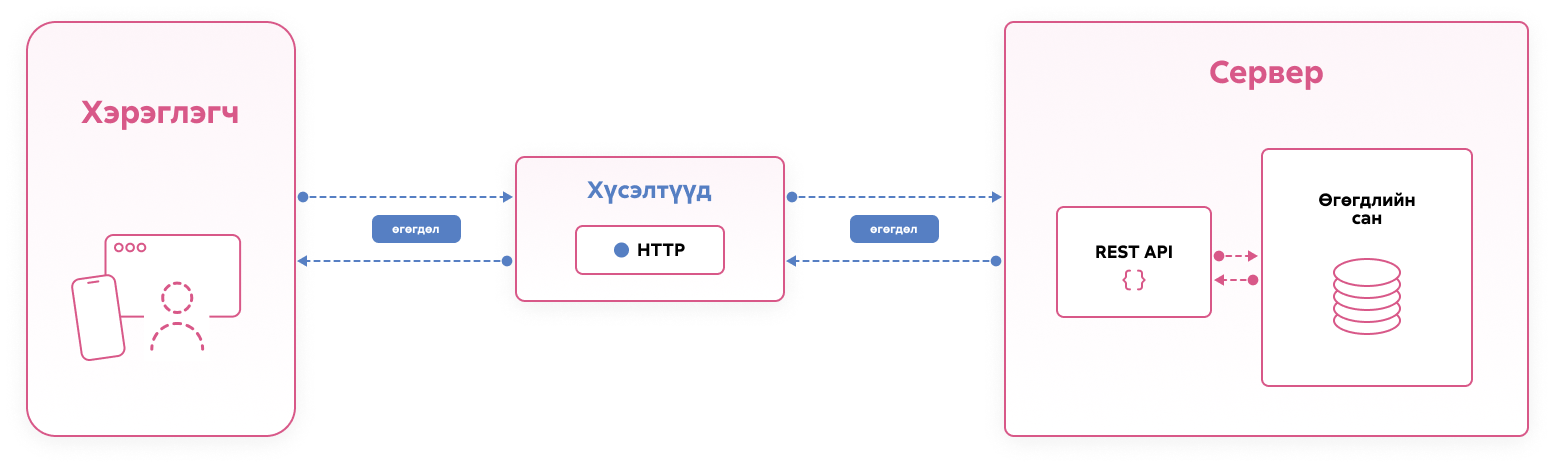
\includegraphics[width=15cm]{images/architecture.png}
	\caption{Three-tier Архитектурын үлгэр загварын дүрслэл}
	\label{fig:architecture}
\end{figure}

\clearpage

Front-end хэсэг Next.js дээр хөгжүүлэлт хийгдэх бол. Харин Back-end хэсэг Express.js болон Firebase дээр хөгжүүлэлт хийгдэнэ.

\begin{figure}[h]
	\centering
	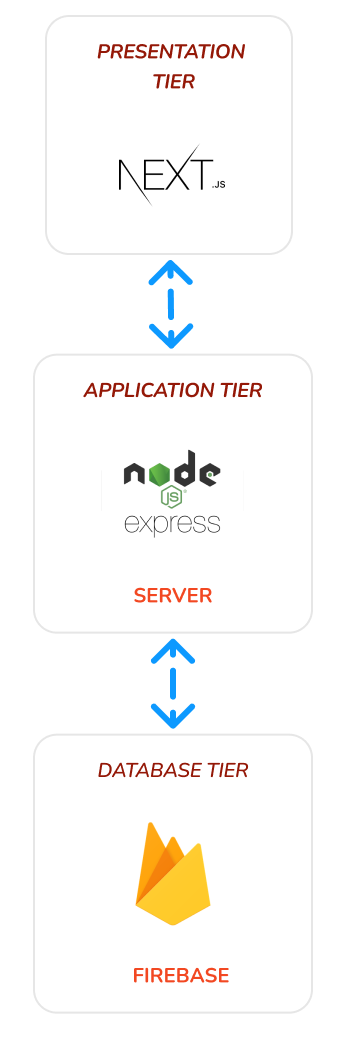
\includegraphics[scale=0.9]{images/imp-diag.png}
	\caption{Хэрэгжүүлэх гэж буй системийн архитектур}
	\label{fig:imp-architecture}
\end{figure}

\pagebreak
\section{Ажлын явцын диаграм}

\subsection{Ажлын явцын диаграм}
\begin{figure}[h]
	\centering
	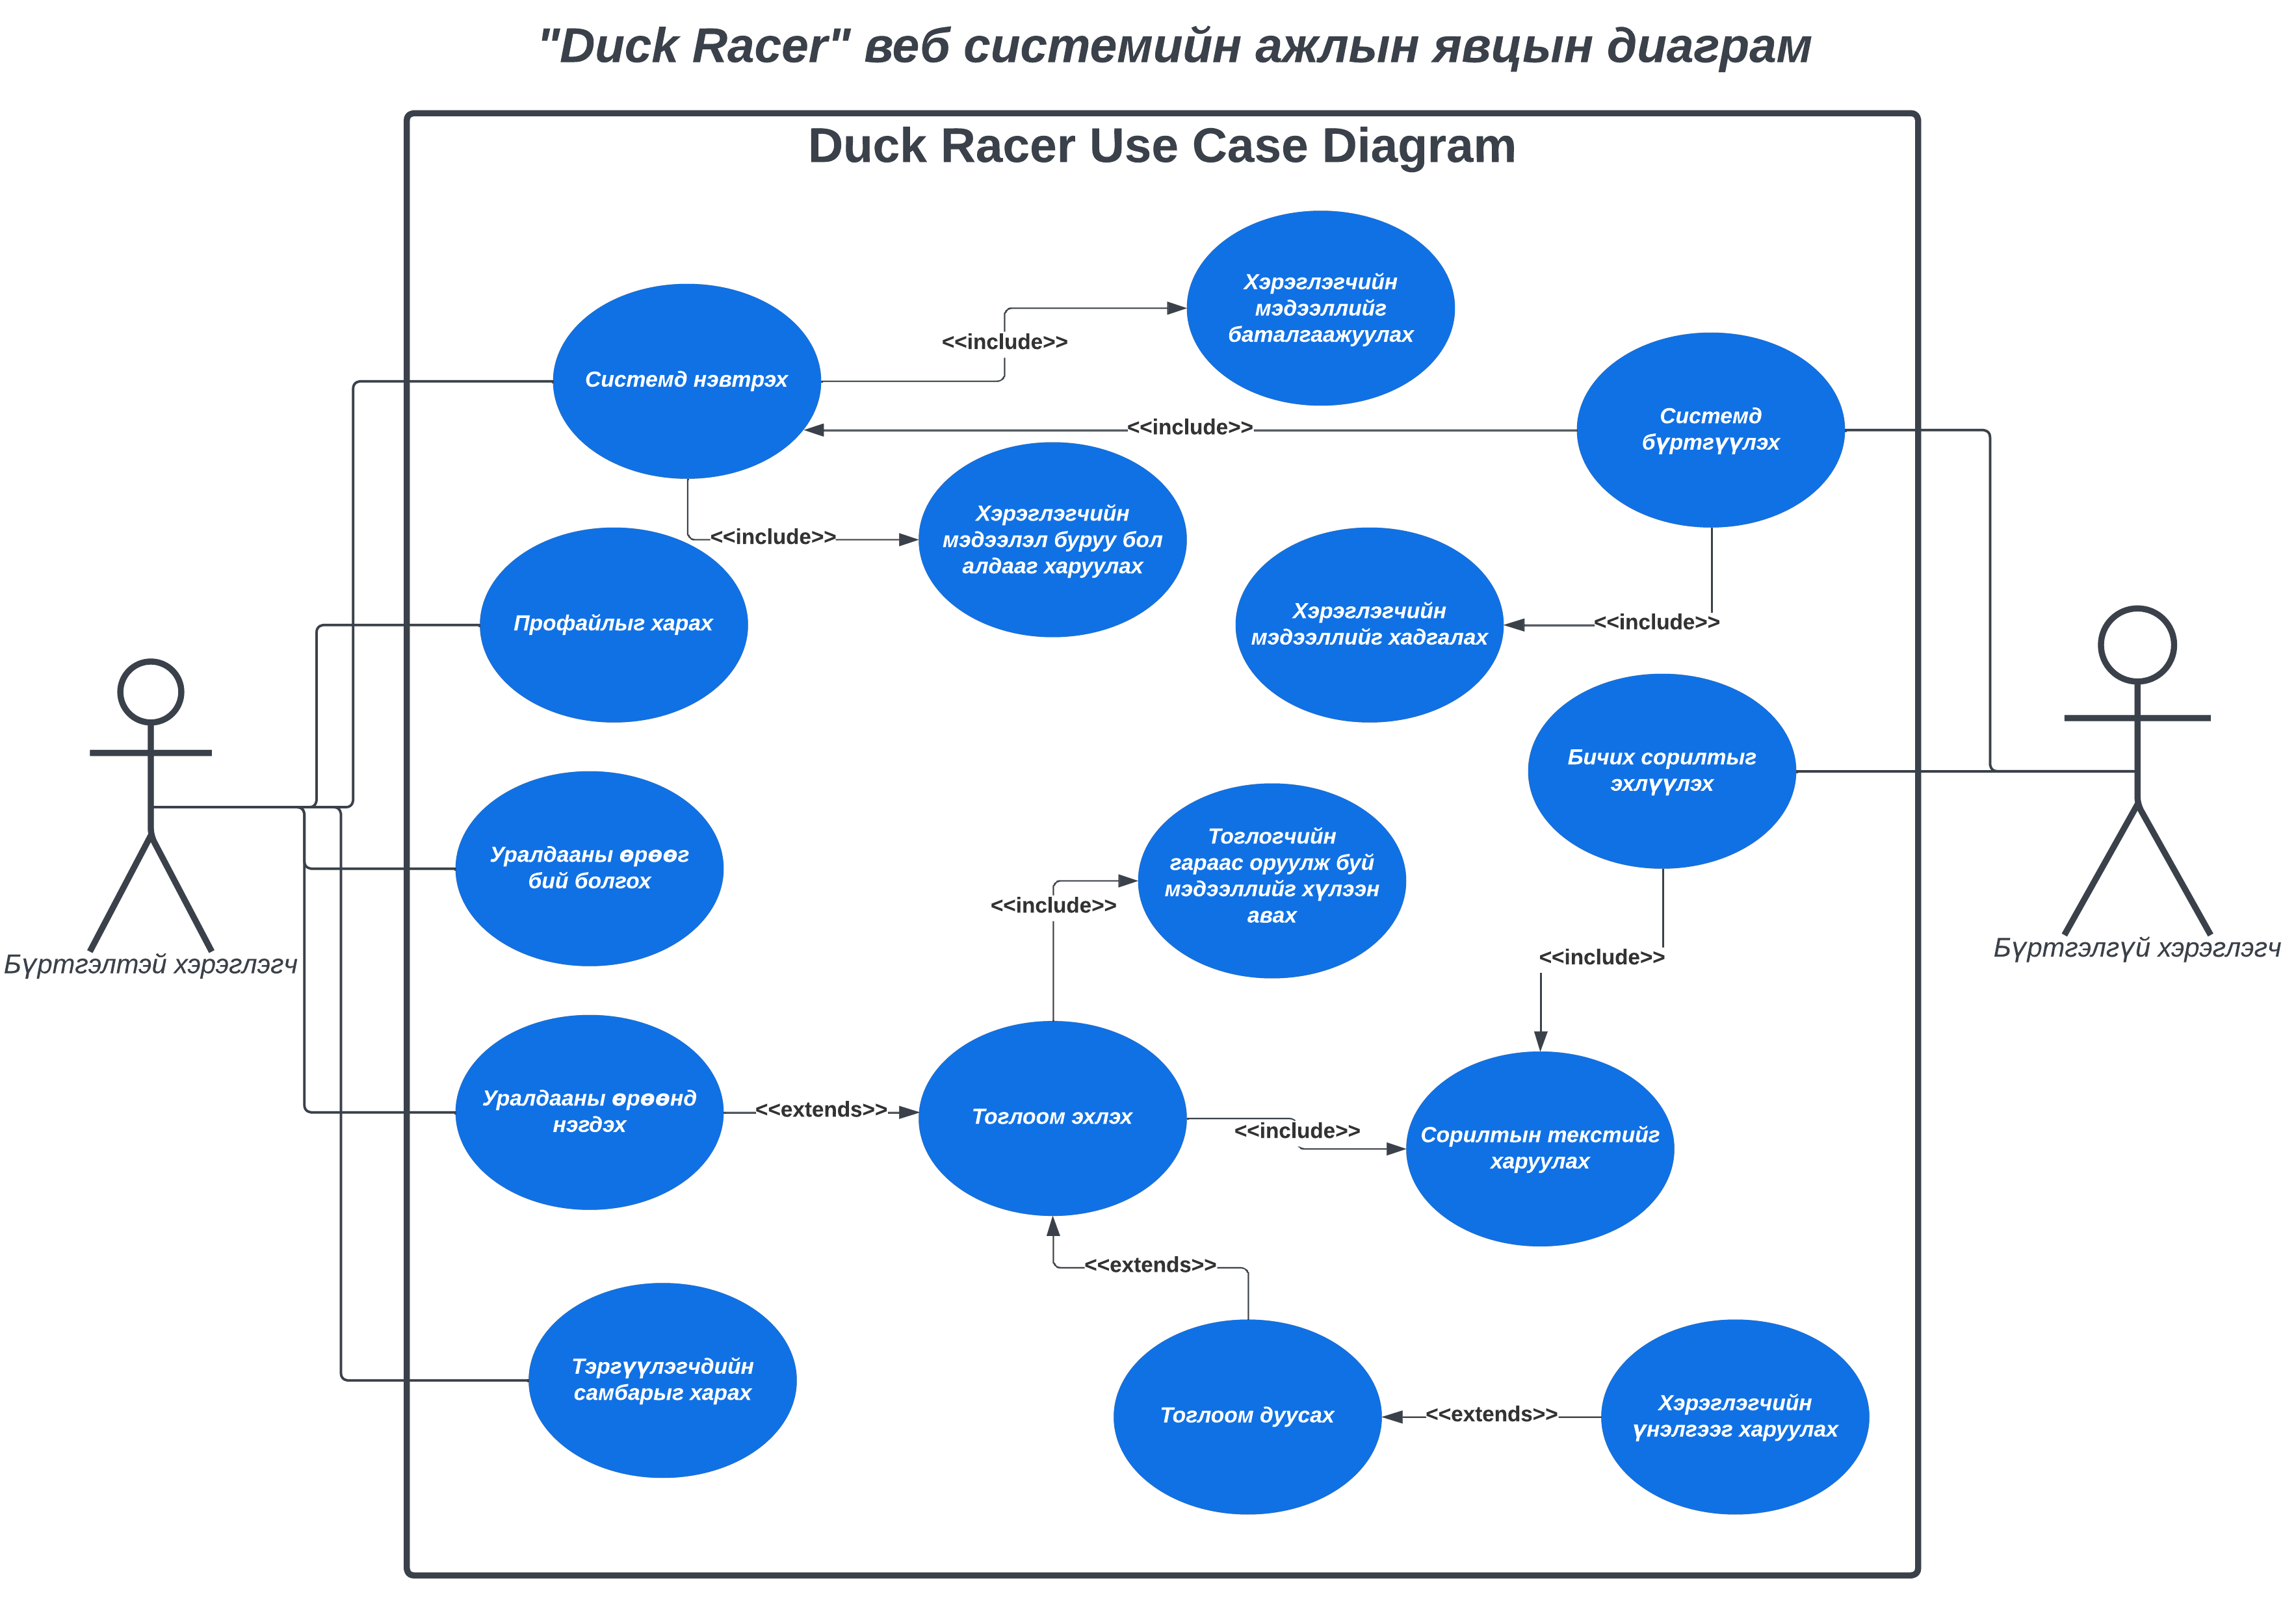
\includegraphics[width=15cm]{images/usecase.png}
	\caption{Ажлын явцын диаграм}
	\label{fig:usecase}
\end{figure}

\textbf{Ажлын явцын диаграмын тайлбар}

\begin{itemize}
	\item \textbf{Нэвтрэх -} Бүртгүүлсэн хэрэглэгч системд хэрэглэгчийн нэр, нууц үгээ оруулан нэвтрэх.
	\item \textbf{Бүртгүүлэх -} Хэрэглэгч бүртгэлгүй хэдий ч манай платформыг бүрэн ашиглах боломжтой. Хэрэв өөрөө веб холбоос оруулахыг хүсвэл хувийн мэдээллээ бөглөж бүртгүүлэх.
	\item \textbf{Хэрэглэгчийн мэдээллийг баталгаажуулах -} Бүртгэгдсэн хэрэглэгч шивэх сорилтынхоо үр дүнг харж, ахиц дэвшлийг нь харж, сайжруулах шаардлагатай хэсгийг тодорхойлох.
	\item \textbf{Хэрэглэгчийн мэдээлэл буруу бол алдааг харуулах -} Бүртгэгдсэн хэрэглэгч шивэх сорилтынхоо үр дүнг харж, ахиц дэвшлийг нь харж, сайжруулах шаардлагатай хэсгийг тодорхойлох.
	\item \textbf{Профайлыг харах -} Бүртгэгдсэн хэрэглэгч өөрийн профайлыг харж шивэх хурд, нарийвчлал болон бусад статистикийг харах.
	\item \textbf{Шивэх сорилтыг эхлүүлэх -} Бүх хэрэглэгч шивэх чадвараа сайжруулахын тулд шивэх сорилтыг эхлүүлэх.
	\item \textbf{Тэргүүлэгчдийн самбарыг харах -} Бүртгүүлсэн хэрэглэгч тэргүүлэгчдийн самбарыг харж бусад хэрэглэгчдийнхээ эсрэг хэрхэн эрэмбэлэгдсэнийг харах.
	\item \textbf{Уралдааны өрөөг бий болгох -} Бүртгүүлсэн хэрэглэгч бусад хэрэглэгчдийг шивэх уралдаанд уралдуулахын тулд уралдааны өрөө үүсгэх.
	\item \textbf{Уралдааны өрөөнд нэгдэх -} Бүртгүүлсэн хэрэглэгч өөр хэрэглэгчийн үүсгэсэн уралдааны өрөөнд нэгдэх.
	\item \textbf{Тоглоом эхлэх -} Өрөөнд нэгдсэний дараагаар уралдааныг эхлүүлэх.
	\item \textbf{Тоглогчийн гараас оруулж буй мэдээллийг хүлээн авах -} Хэрэглэгчийн мэдээллийг серверлүү илгээх.
	\item \textbf{Сорилтын текстийг харуулах -} Баазаас текстийг татан авч харуулах.
	\item \textbf{Тоглоом дуусах -} Тодорхой хугацааны дараа уралдааныг дуусгах.
	\item \textbf{Хэрэглэгчийн  үнэлгээг харуулах -} Хэрэглэгчийн мэдээллийг боловсруулж мэдээллийг харуулах.
	\item \textbf{Хэрэглэгчийн мэдээллийг хадгалах -} Тоглоом дууссаны дараагаар хэрэглэгчийн мэдээллийг боловсруулж мэдээллийг хадгалах.
\end{itemize}

\pagebreak
\section{UX/UI дизайн}

Өмнөх бүлэгт хийсэн судалгааны зорилго бол хэрэглэгчдэд ээлтэй, харагдахуйц харагдахуйц интерфэйсийг бий болгох явдал байсан.

\begin{itemize}
	\item хэрэглэгчдийн хэрэгцээ, хүсэл сонирхолд нарийвчлан дүн шинжилгээ хийж, бидний дизайн, хөгжүүлэлт зорилтот хэрэглэгчдэдээ хамгийн сайн туршлагыг бий болгоход чиглэсэн.
	\item Шинэлэг, мэдрэмжтэй хэрэглэгчийн интерфэйс (UI) загварыг бий болгоход хүчин чармайлтаа зориулсан.
	\item Дизайнаас хөгжүүлэлт рүү жигд шилжихийг хөнгөвчлөхийн тулд UI дизайнтай нягт уялдуулах замаар урд талын хөгжүүлэлтийн процессыг хурдасгасан.
\end{itemize}

\subsection{Эхний загвар}

\textbf{Эхний Wireframe загварыг гаргаж Prototype хувилбар бүтээсэн нь}

Вебийн гол процессийг илэрхийлэх 4 зургийг орууллаа. Бусад хэсгийг хавсралтаас \footnote{Зурсан интерфейс дизайн \url{https://shorturl.at/djwAT}} үзэх боломжтой.

\begin{figure}[h]
	\centering
	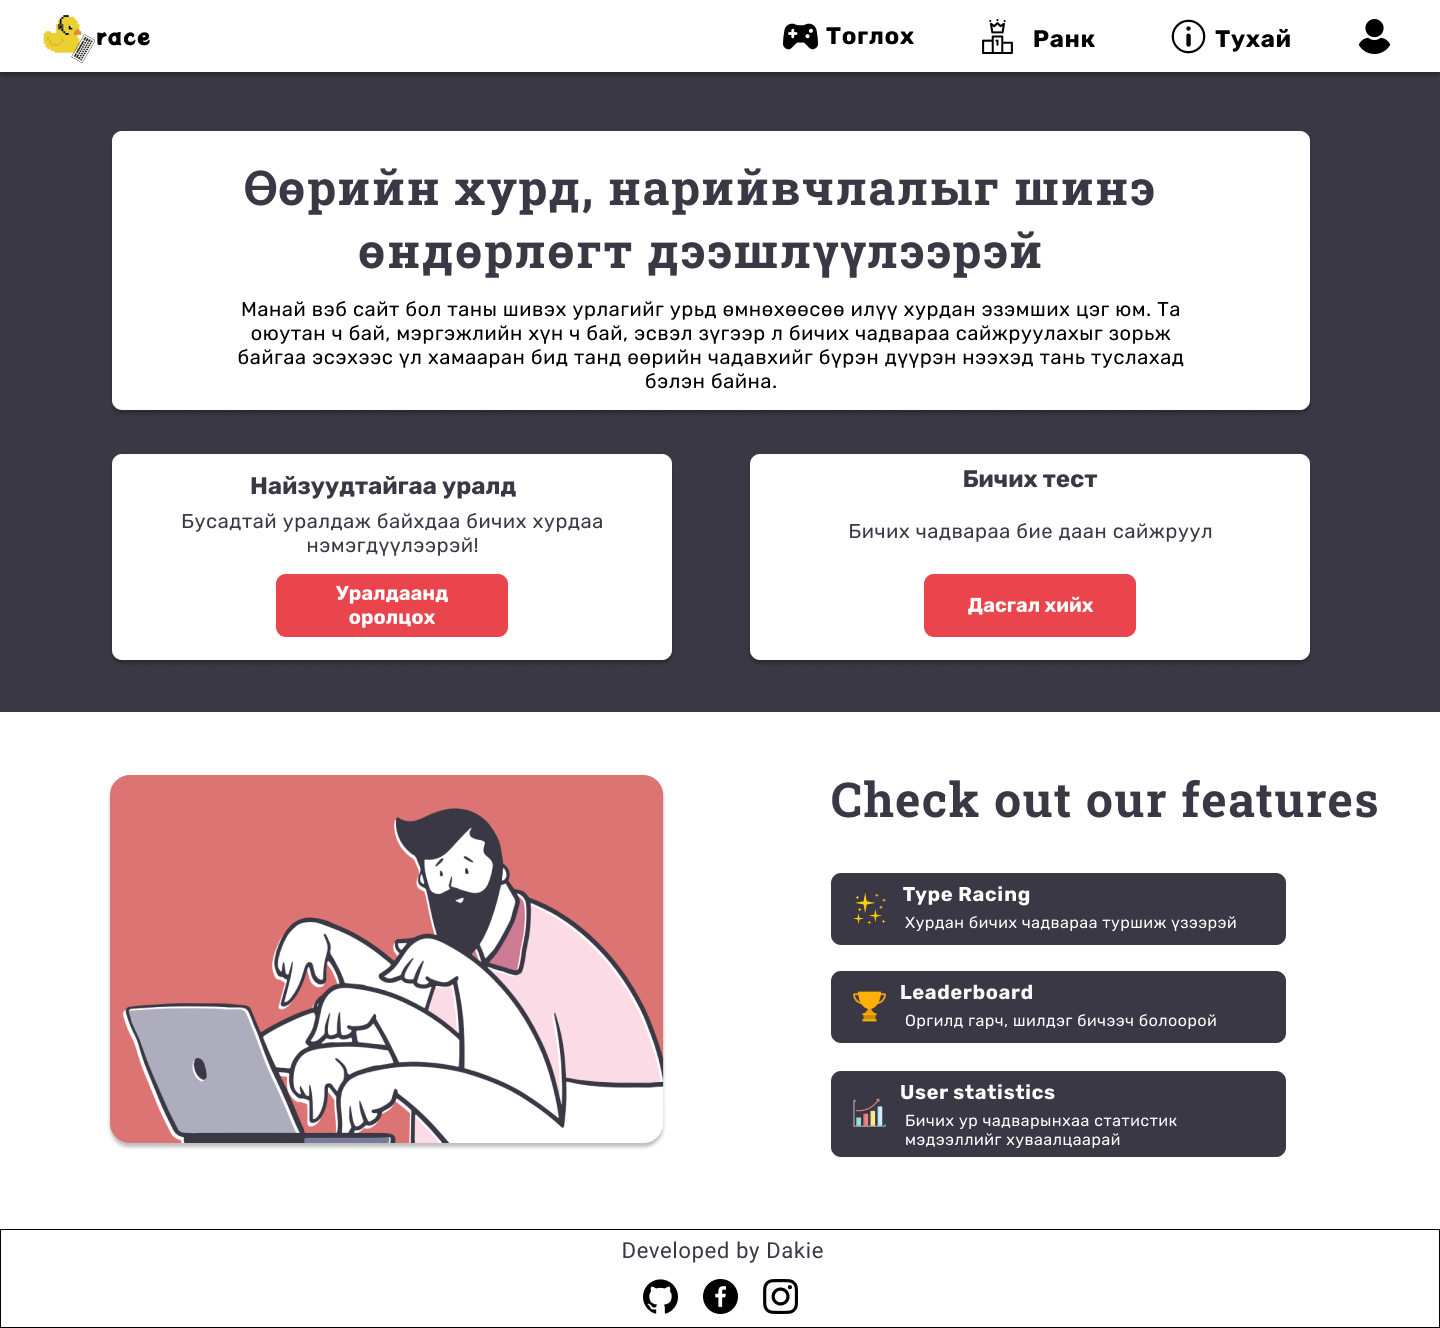
\includegraphics[width=10cm]{images/interfaces/ver1/mainpage.png}
	\caption{Нүүр хуудас}
	\label{fig:interface-v1-01}
\end{figure}

\begin{figure}[h]
	\centering
	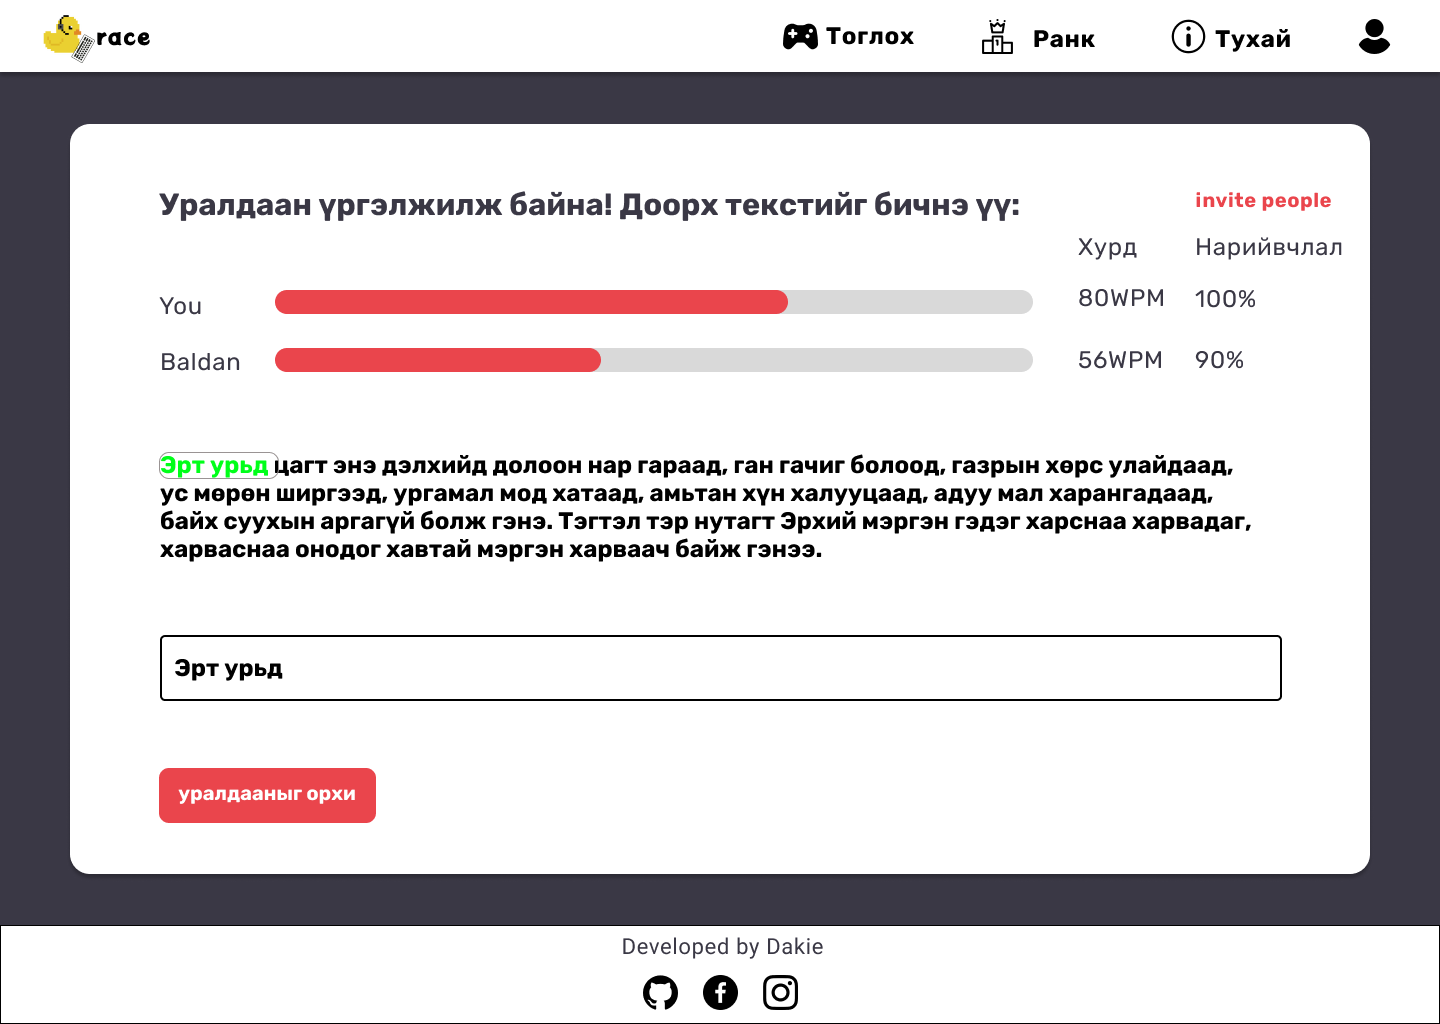
\includegraphics[width=10cm]{images/interfaces/ver1/playpage.png}
	\caption{Холбоосуудаа оруулах форм}
	\label{fig:interface-v1-02}
\end{figure}

\begin{figure}[h]
	\centering
	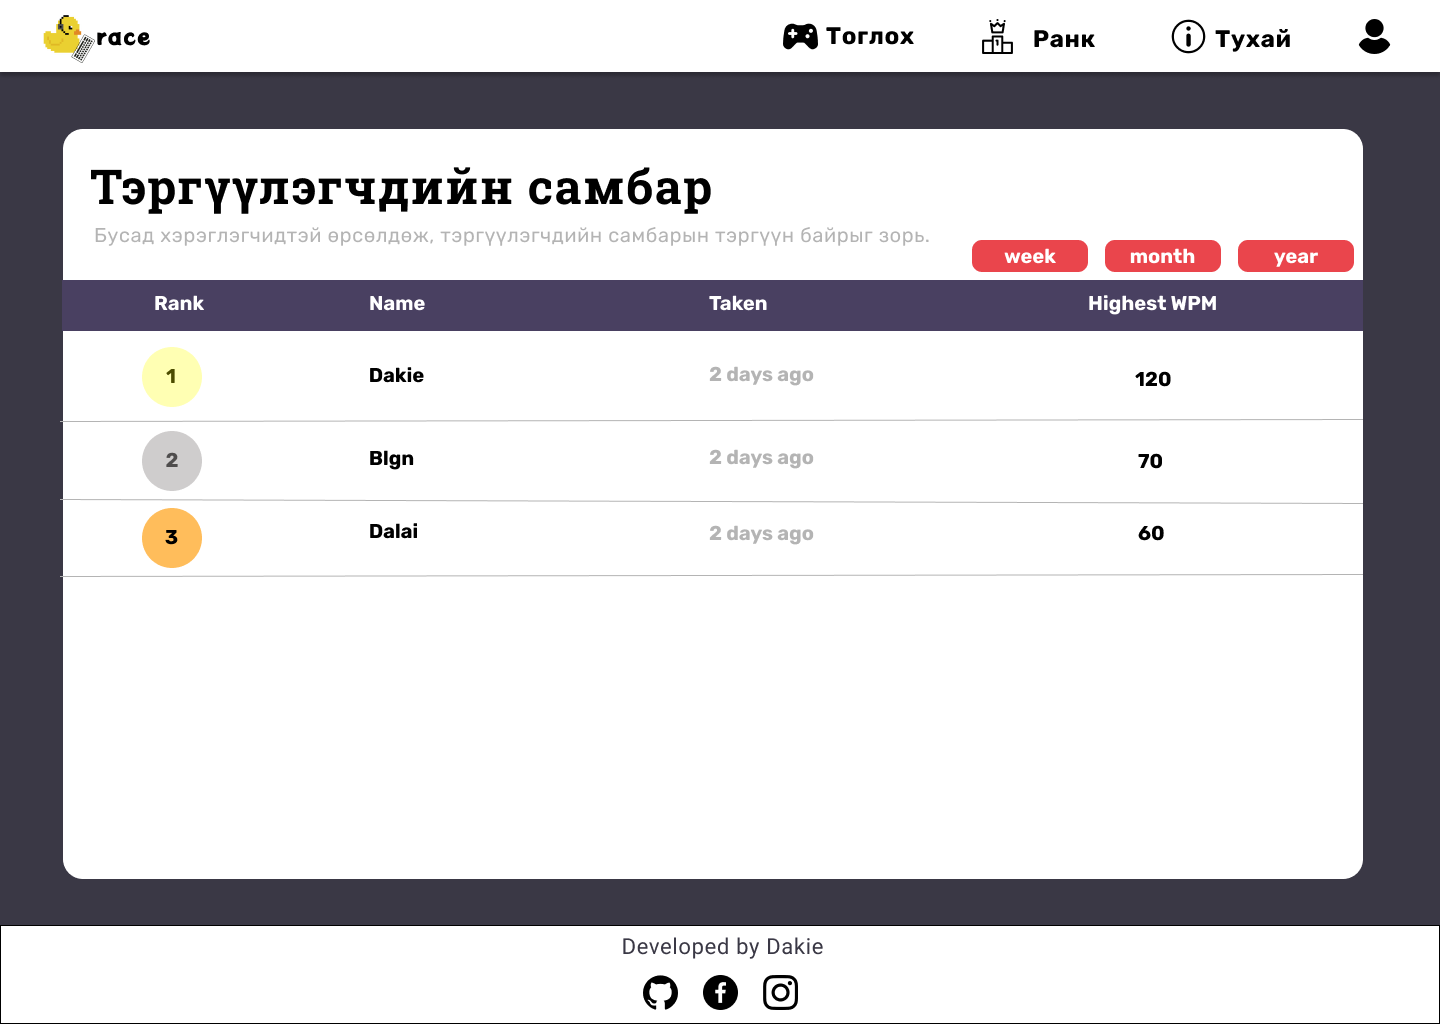
\includegraphics[width=10cm]{images/interfaces/ver1/leaderboard.png}
	\caption{Оруулсан холбоосуудыг нийтлэсний дараах хуудас}
	\label{fig:interface-v1-03}
\end{figure}

\begin{figure}[h]
	\centering
	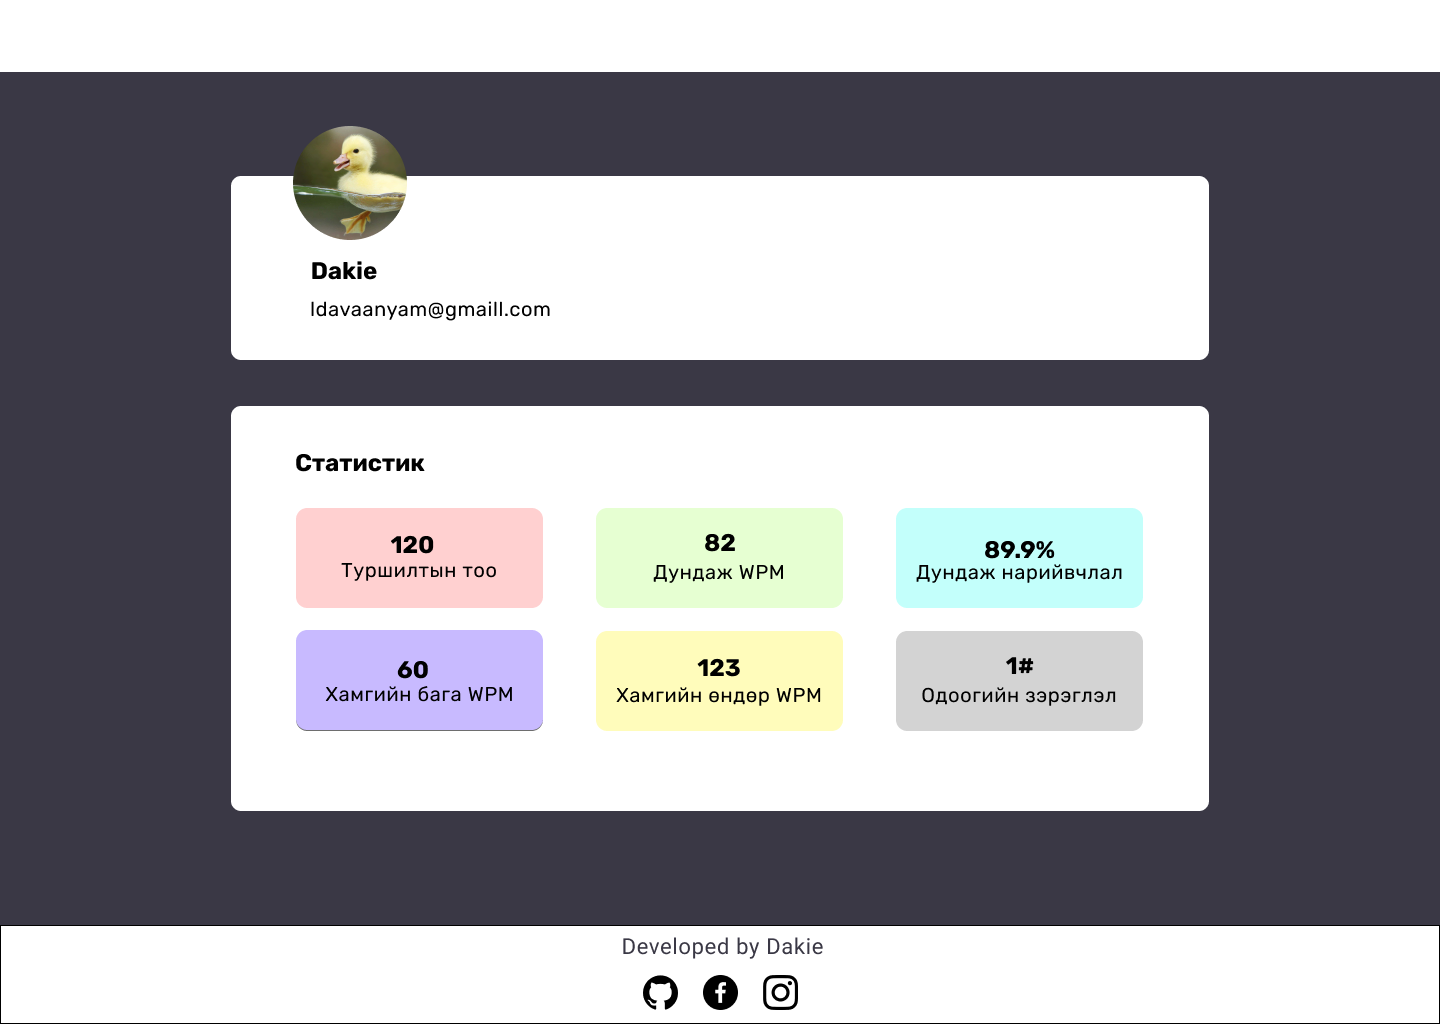
\includegraphics[width=10cm]{images/interfaces/ver1/profilepage.png}
	\caption{Оруулсан нийтлэл бусад хүмүүст харагдах байдал}
	\label{fig:interface-v1-04}
\end{figure}

\clearpage
% \textbf{Prototype хувилбар дээрээ Usability туршилт хийсэн нь}

% Дараа нь Prototype хувилбар дээрээ Usability буюу хэрэглэхэд тухтай байдлын туршилтыг сонгож авсан хоёр хэрэглэгч дээрээ хийлгэж уг гаргасан дизайн дээрх үүссэн асуудлыг тодорхойлж, хэрэглэгчээс санал хүсэлтийг аван дараагийн гаргах дизайныхаа ерөнхий шаардлагуудыг тодорхойлов. Үүнээс дурдвал:

% \begin{itemize}
% 	\item UI загварын хувьд концептийг дахин сайжруулах
% 	\item Бусад хүмүүсийн оруулсан холбоосыг нийтэд нь харуулах
% 	\item Оруулж буй холбоосыг ангилалтай байлгах
% 	\item Платформ дээр бүртгэлтэй бусад хэрэглэгчдийг харуулах
% \end{itemize}

% Иймд уг шаардлага дээрээ үндэслэн эцсийн байдлаар вебийнхээ UX/UI дизайныг гаргах шаардлагатай.

% \textbf{Redesign буюу зурсан дизайнаа дахин сайжруулсан нь}

% UX/UI гүйцэтгэлийн хамгийн сүүлийн шатанд нийт 12 хуудас дизайныг \footnote{UX/UI дизайны сүүлийн хувилбар \url{https://www.figma.com/proto/EL2nOGmToBRVxHNuZwH661}} холбож зурсан ба өмнөх дизайны процесстой адилаар Prototype хувилбар гаргаж эцсийн хэрэглэгчдээрээ Usability туршилтыг хийж дараагийн шат болох код хөгжүүлэлтийн шатыг эхлүүлэхэд бэлэн боллоо. Нийт зурсан хуудсаасаа 6 хуудсыг онцлон харуулж, User Expierence дизайныхаа шийдлийг тайлбарлалаа. Бусад зурсан хуудсыг доор байгаа хавсралтаас харах боломжтой. 

% \begin{figure}[h]
% 	\centering
% 	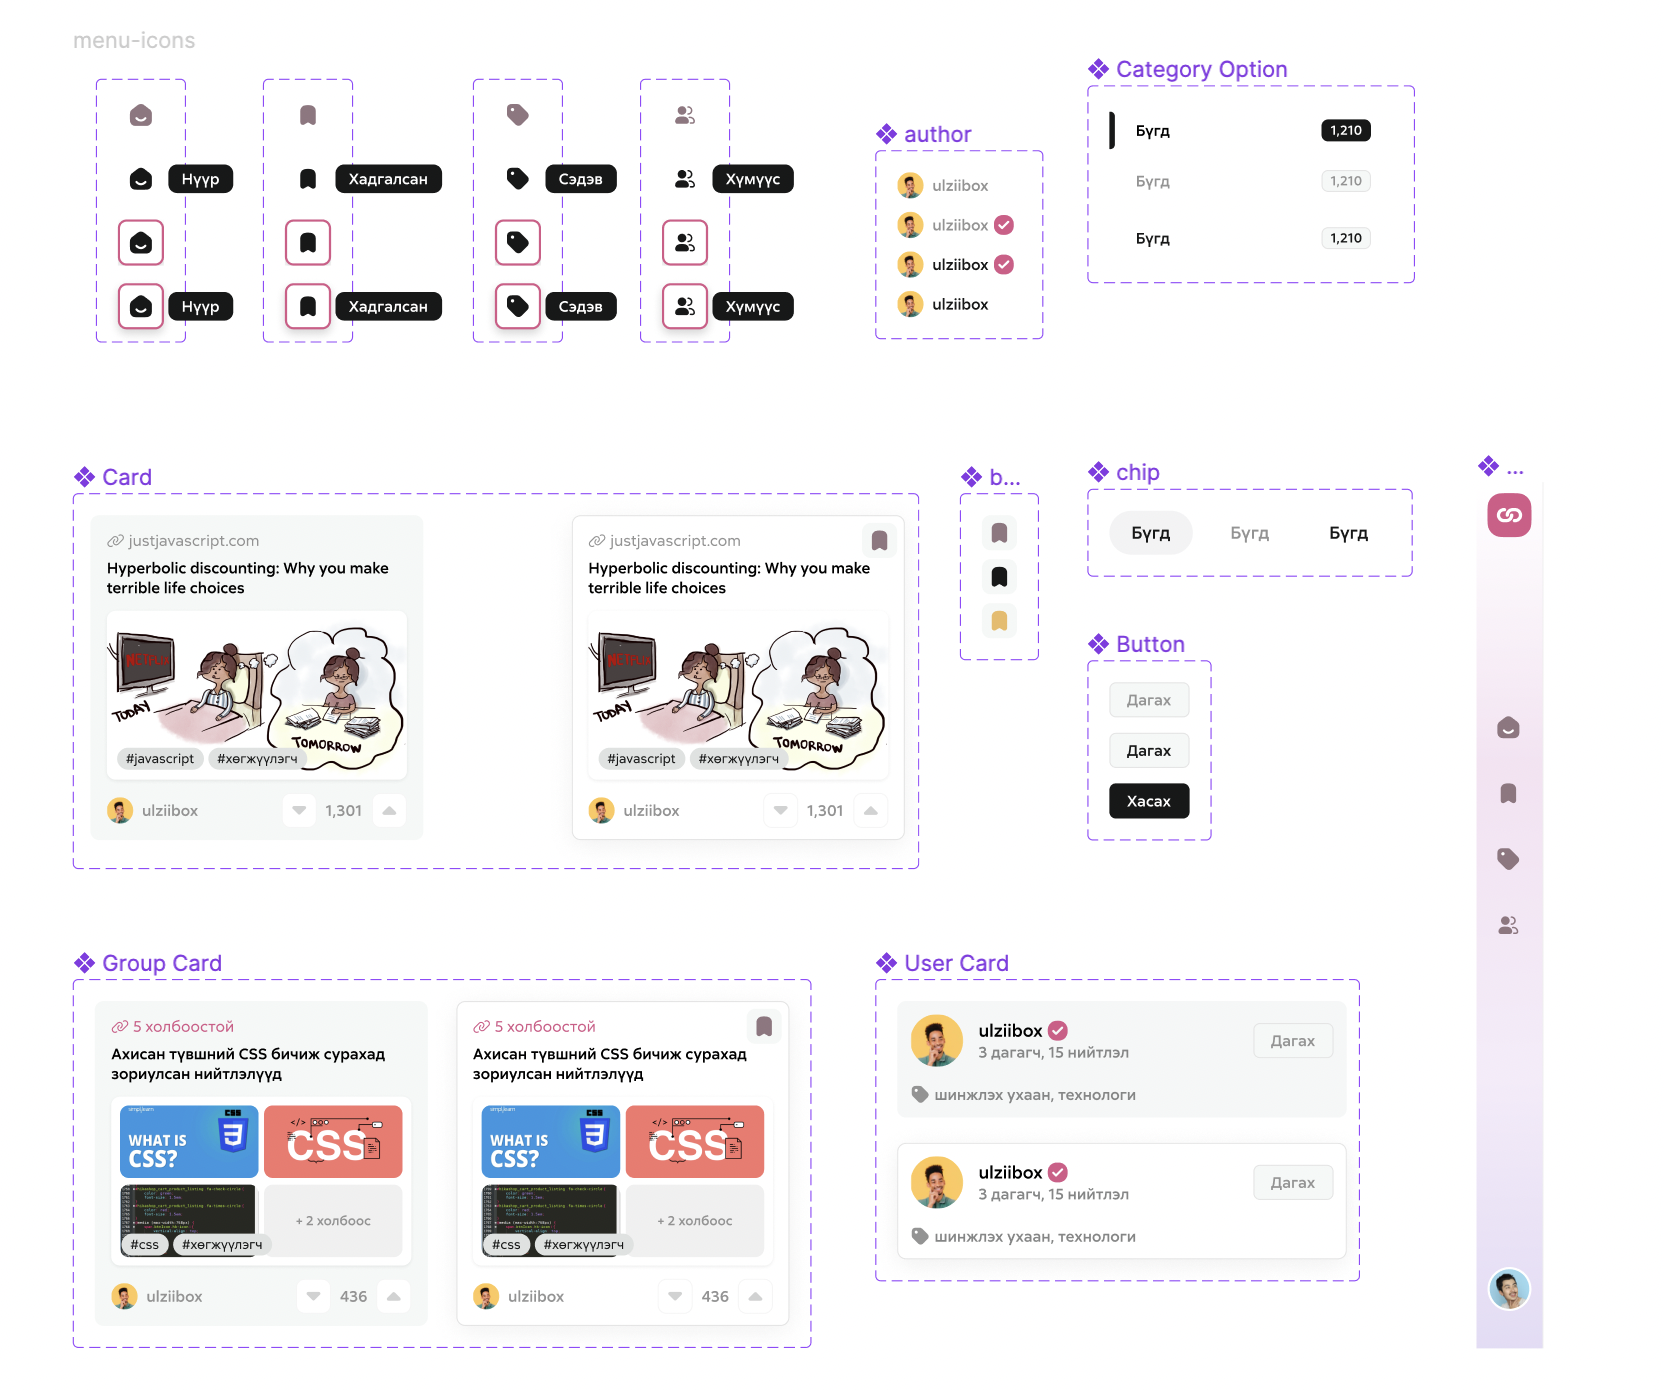
\includegraphics[width=10cm]{images/interfaces/components.png}
% 	\caption{Ашигласан компонентуудын жишээ}
% 	\label{fig:component}
% \end{figure}

% \begin{figure}[h]
% 	\centering
% 	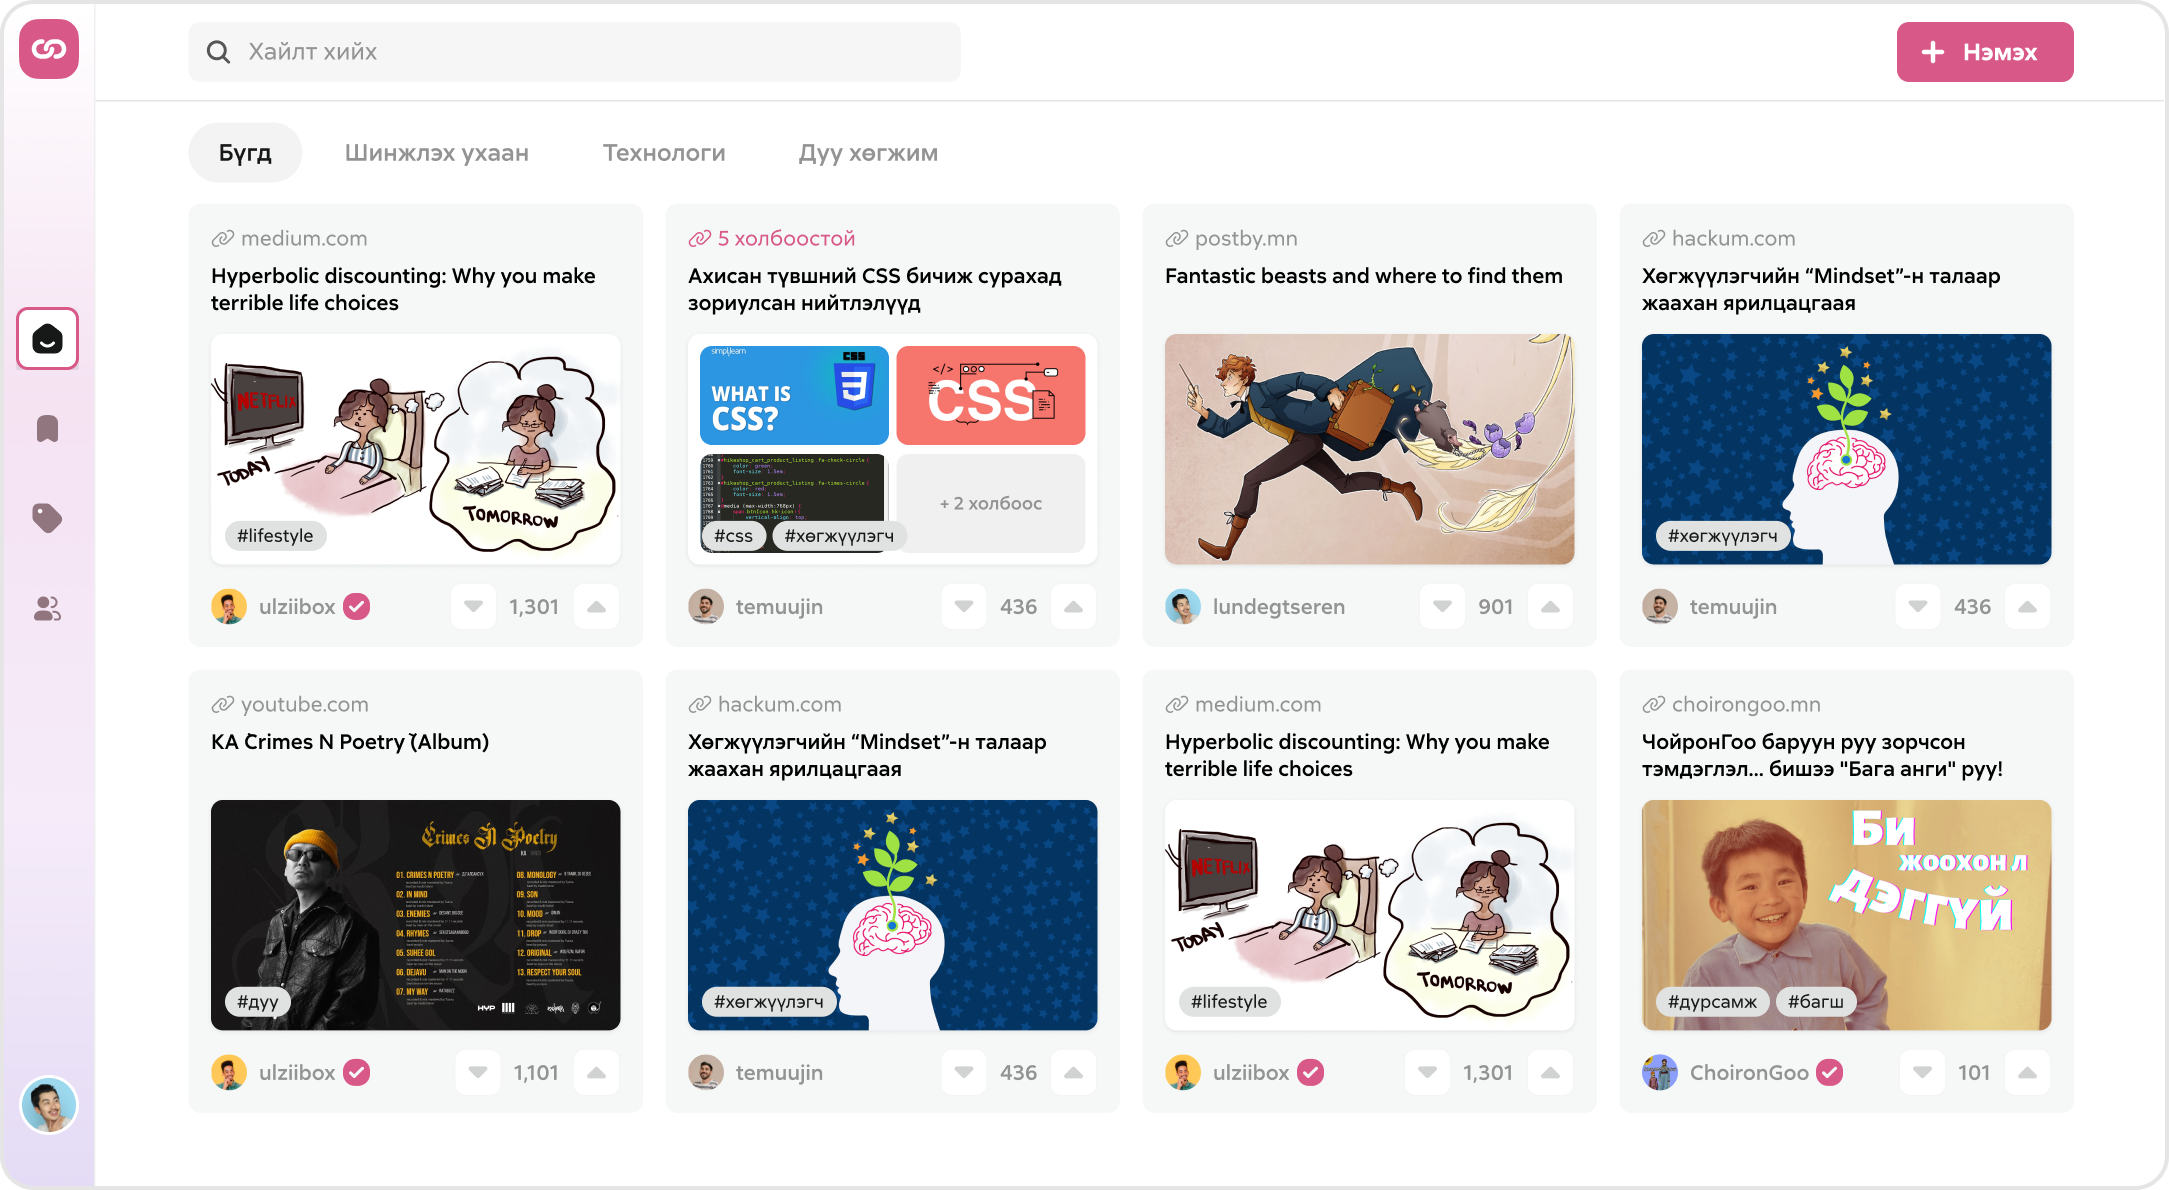
\includegraphics[width=10cm]{images/interfaces/home-screen.png}
% 	\caption{Нэвтэрсний дараах нүүр хуудас}
% 	\label{fig:homescreen}
% \end{figure}

% \begin{figure}[h]
% 	\centering
% 	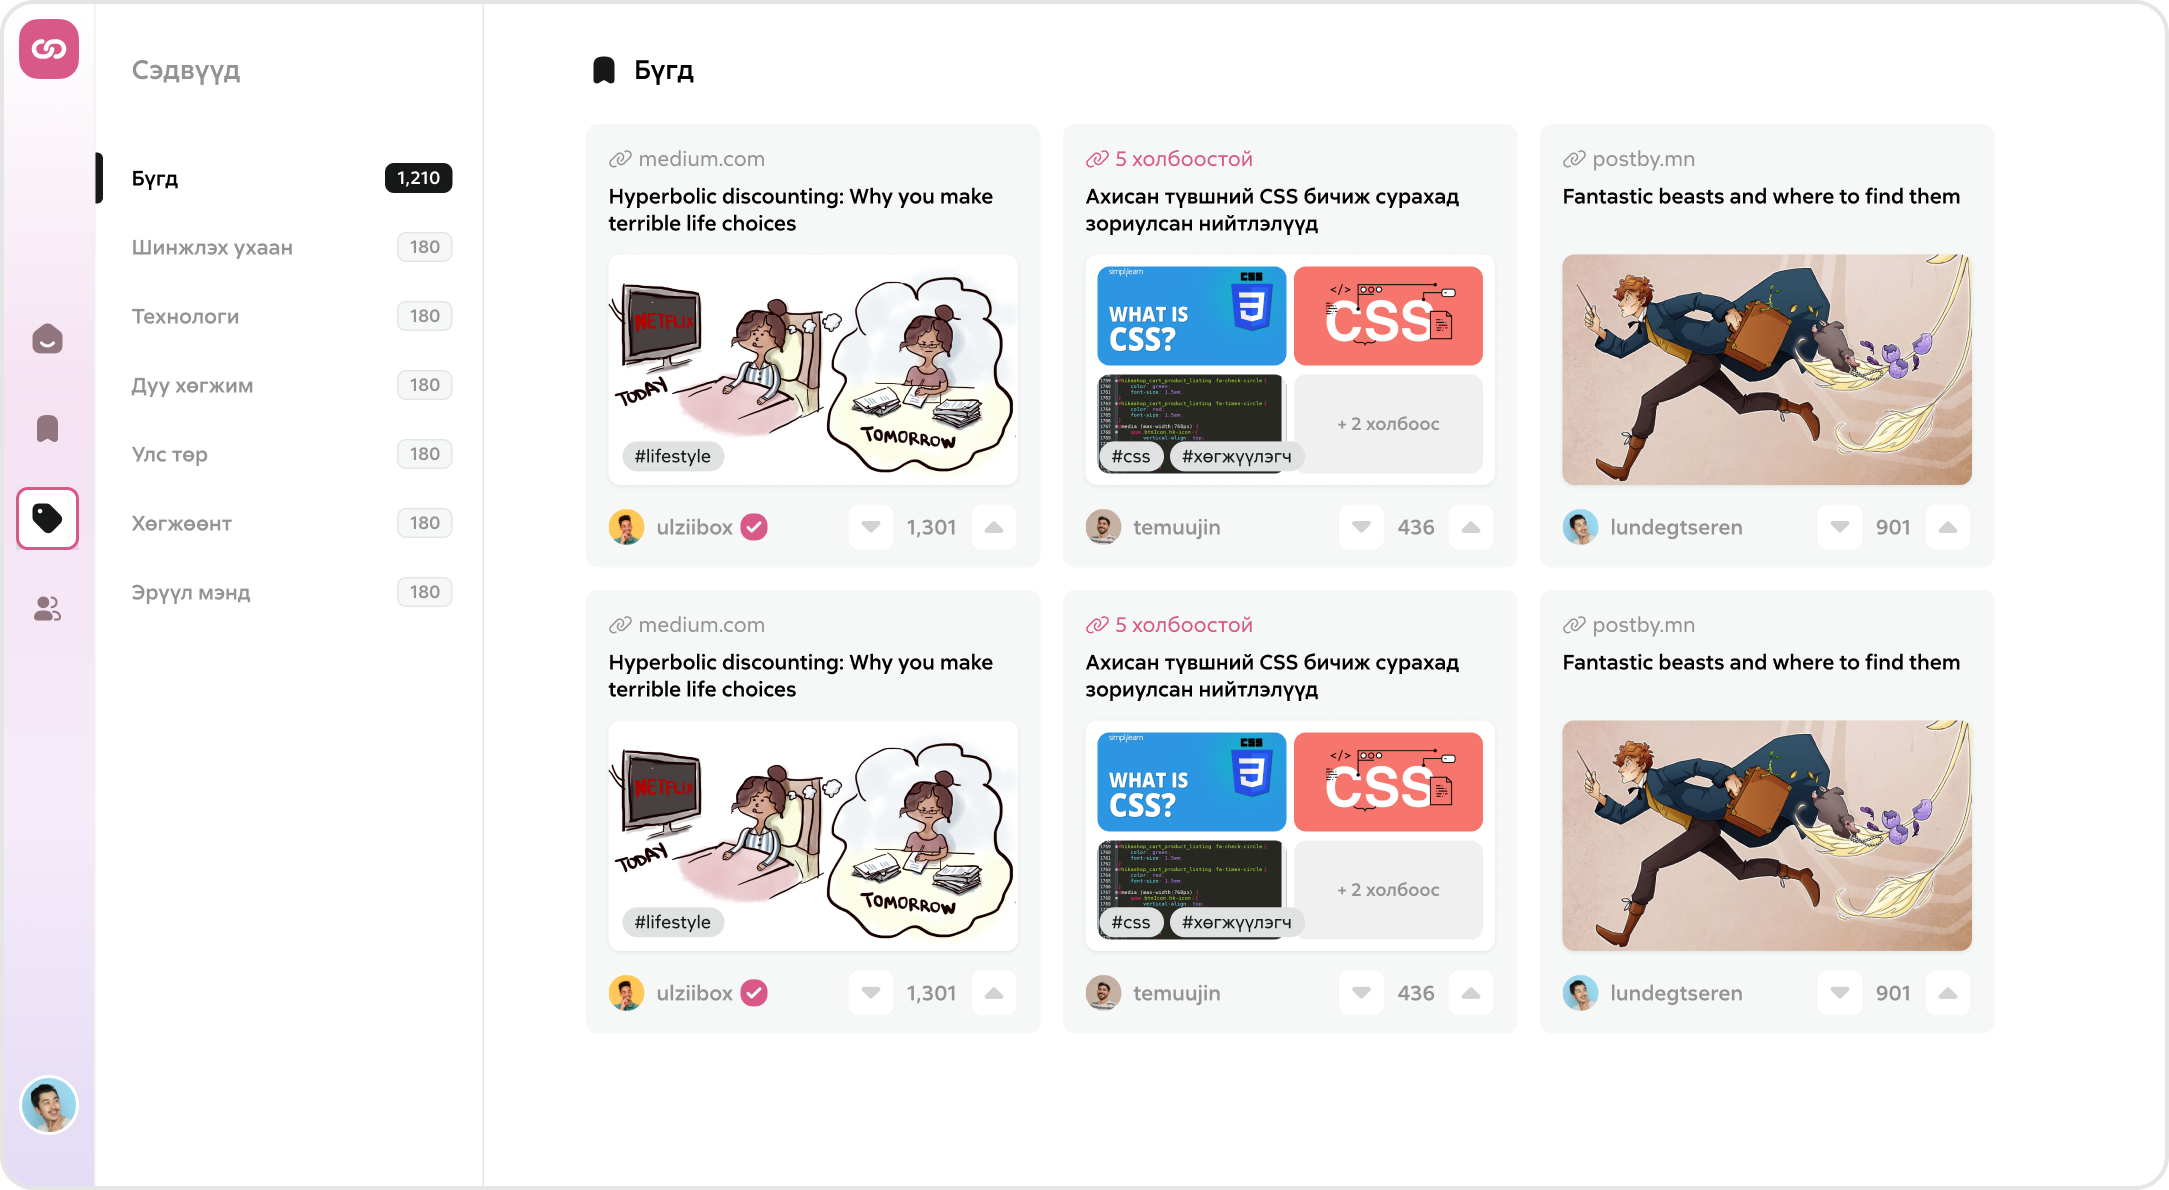
\includegraphics[width=10cm]{images/interfaces/topics.png}
% 	\caption{Бүх холбоосуудыг төрлөөр нь шүүж харах хуудас}
% 	\label{fig:topics}
% \end{figure}

% \begin{figure}[h]
% 	\centering
% 	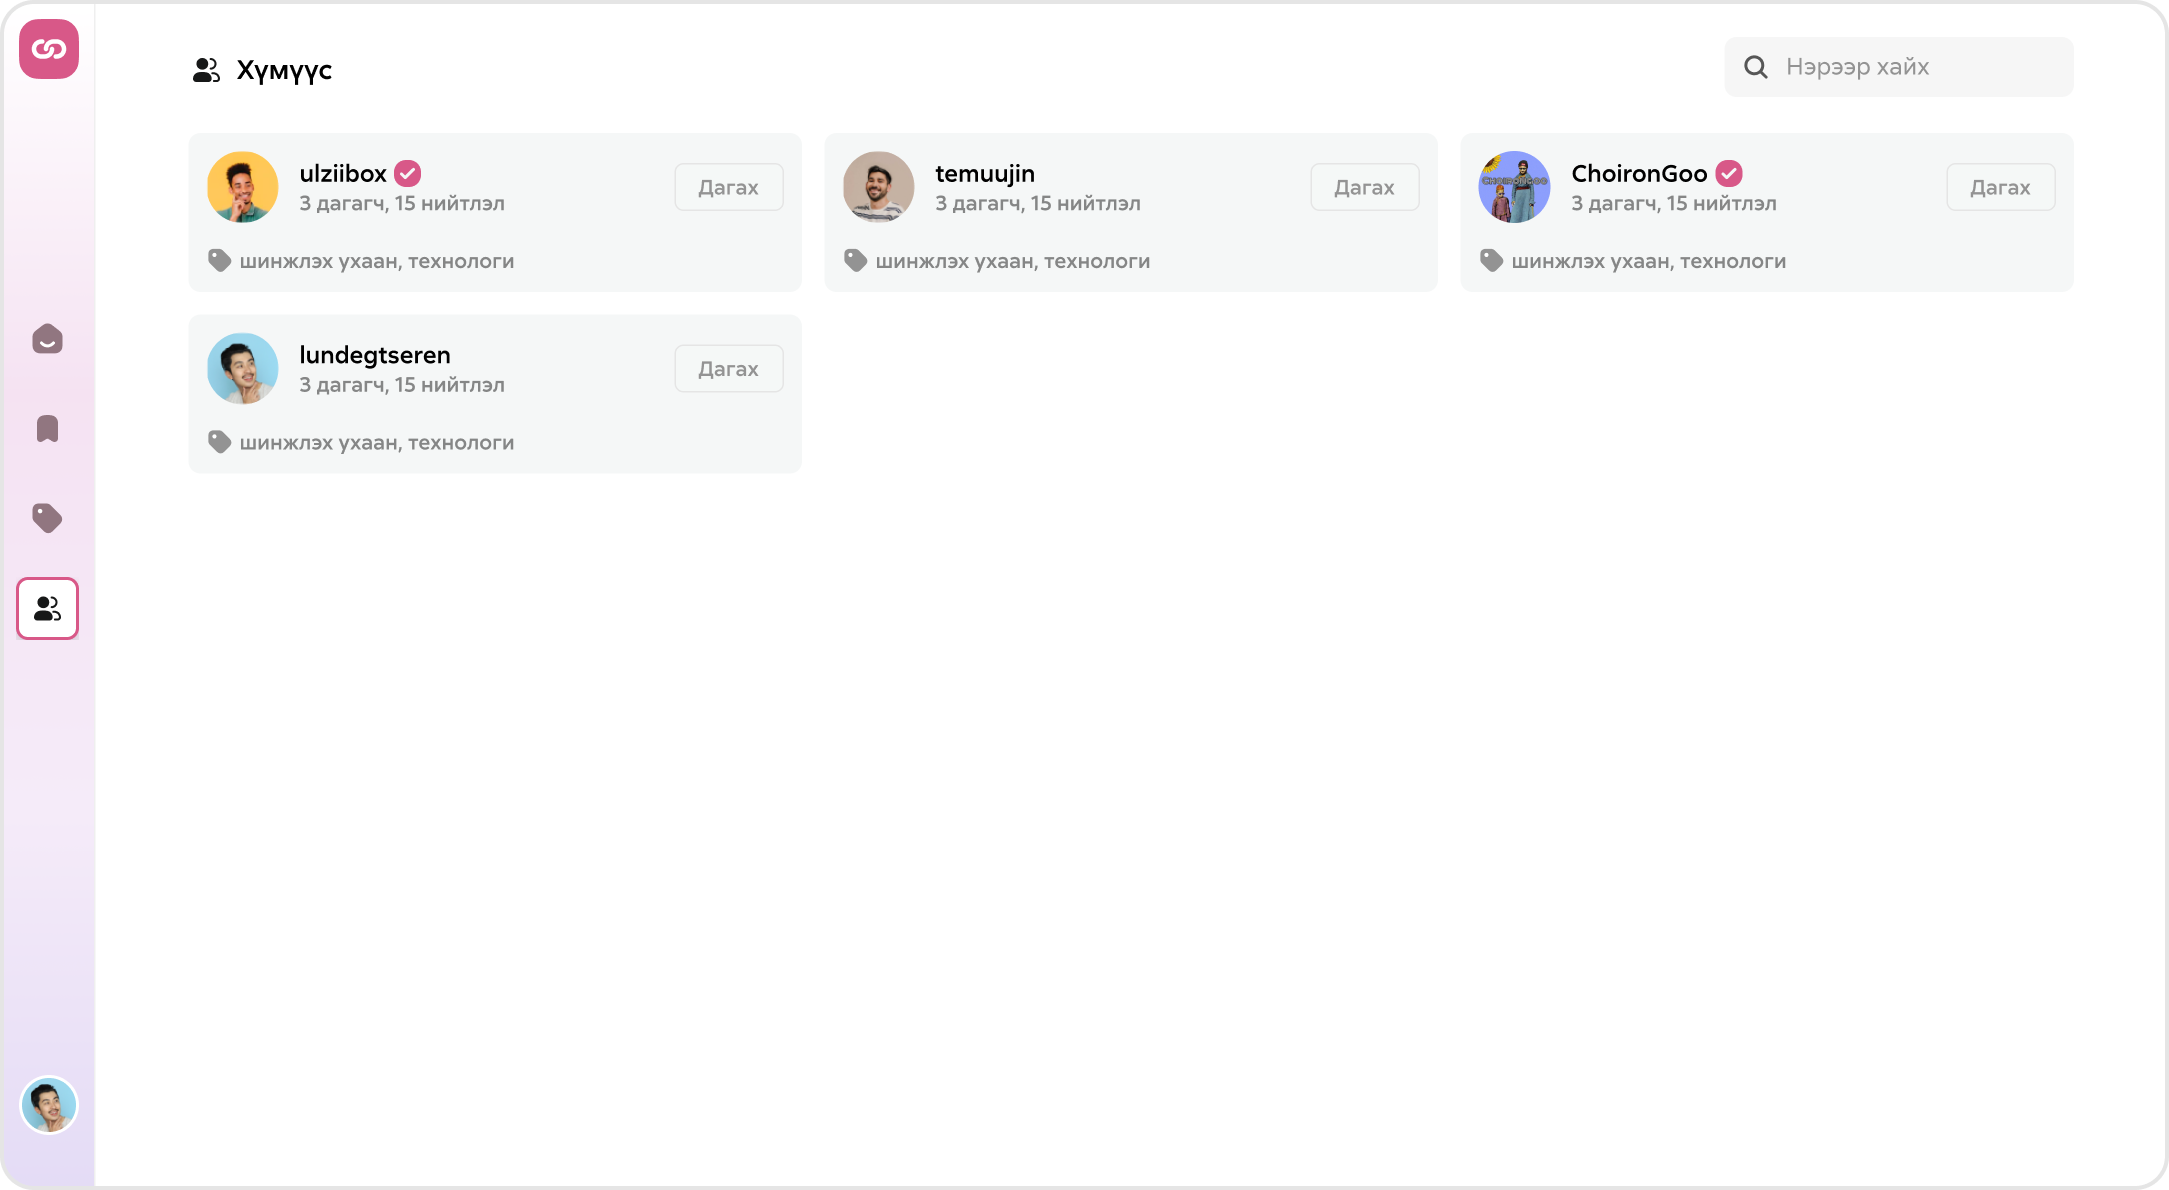
\includegraphics[width=10cm]{images/interfaces/people.png}
% 	\caption{Хэрэглэгчдийн жагсаалт харагдах хуудас}
% 	\label{fig:people}
% \end{figure}

% \begin{figure}[h]
% 	\centering
% 	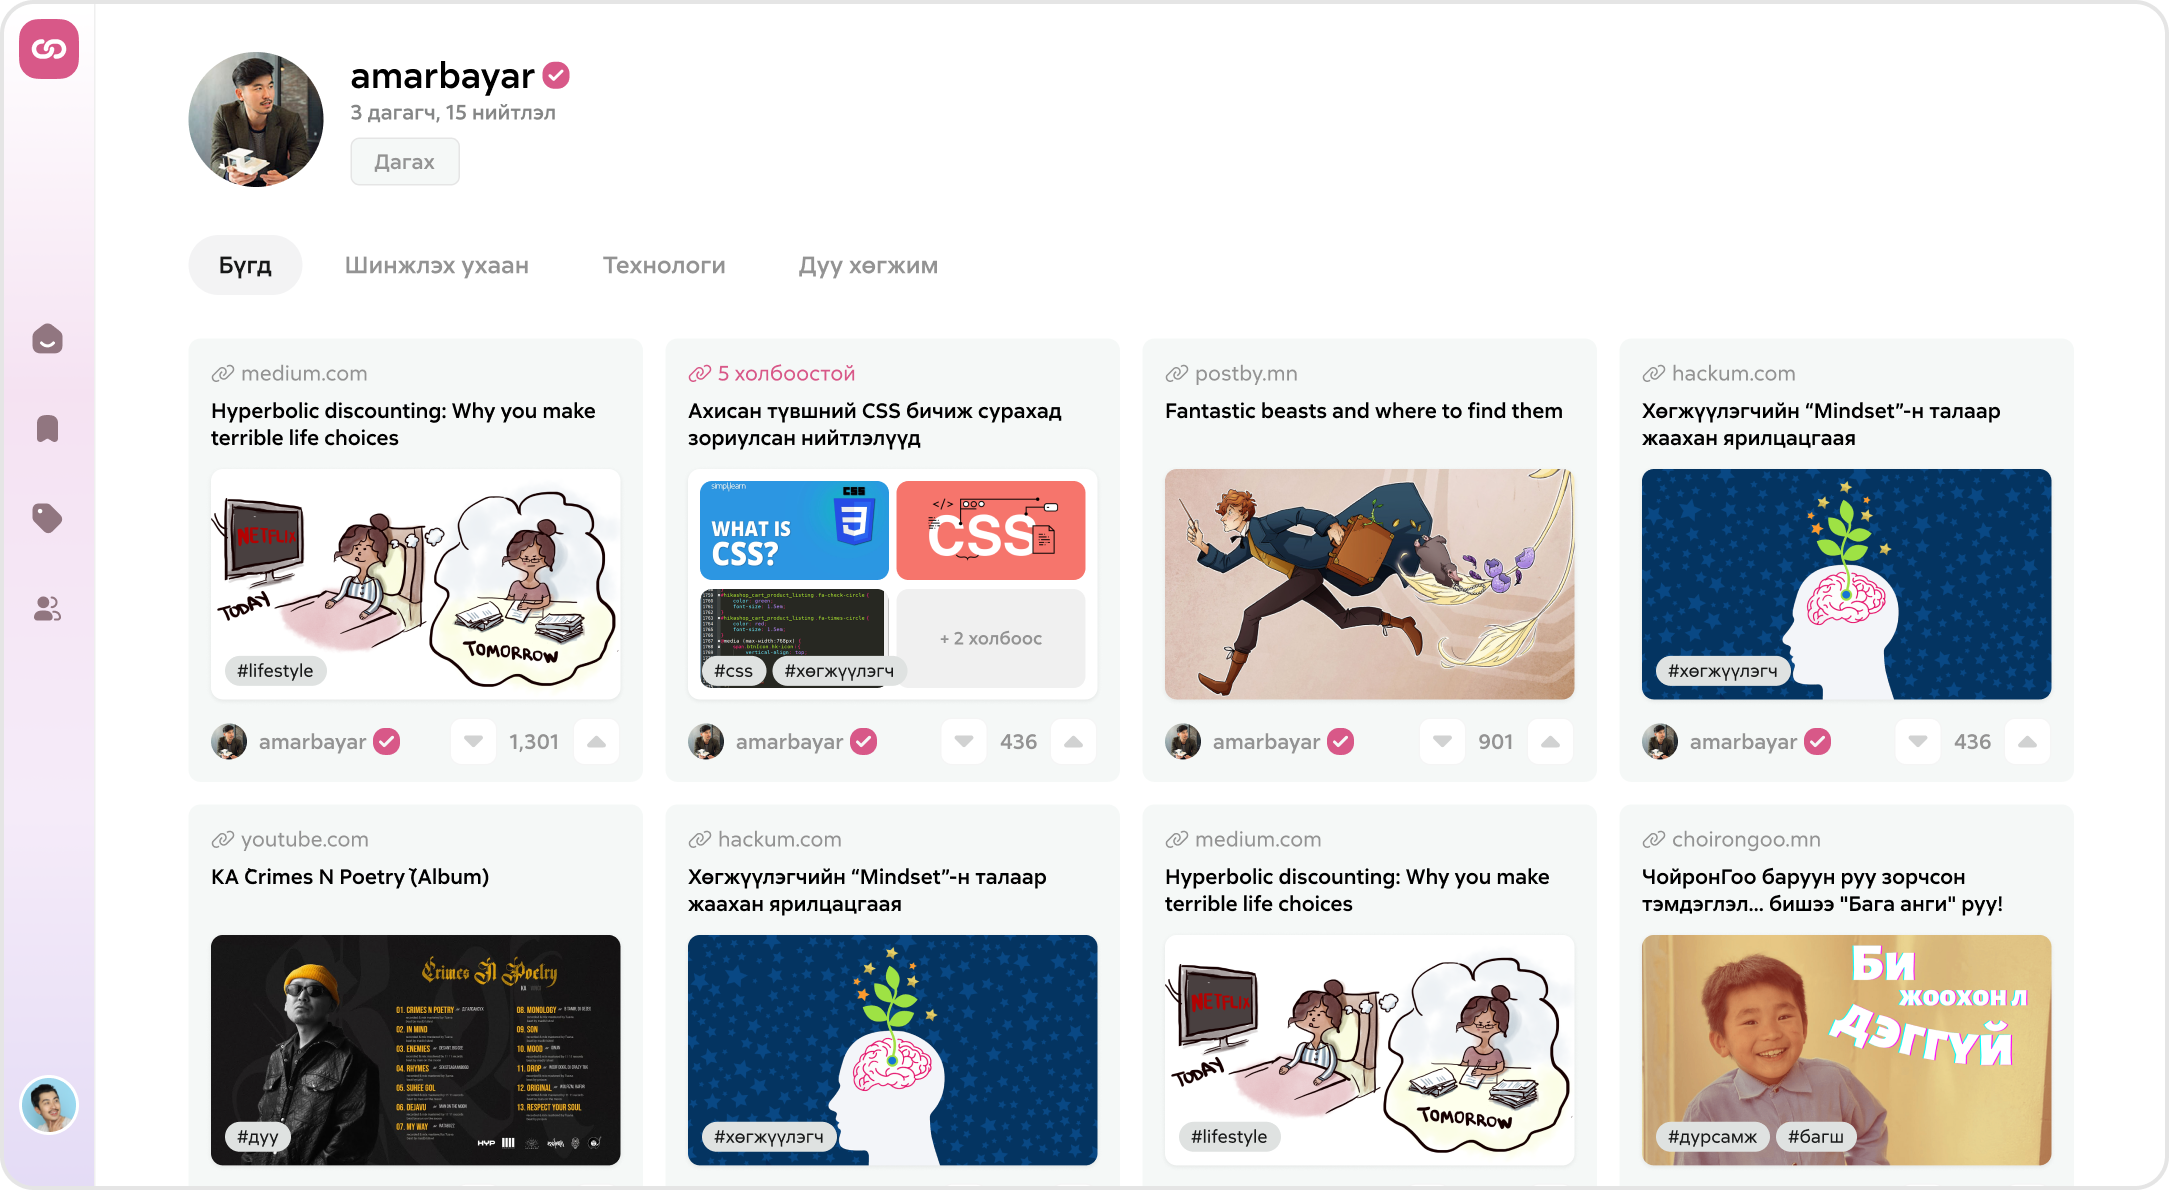
\includegraphics[width=10cm]{images/interfaces/profile.png}
% 	\caption{Бусдын профайлыг харах хуудас}
% 	\label{fig:profile}
% \end{figure}

% \begin{figure}[h]
% 	\centering
% 	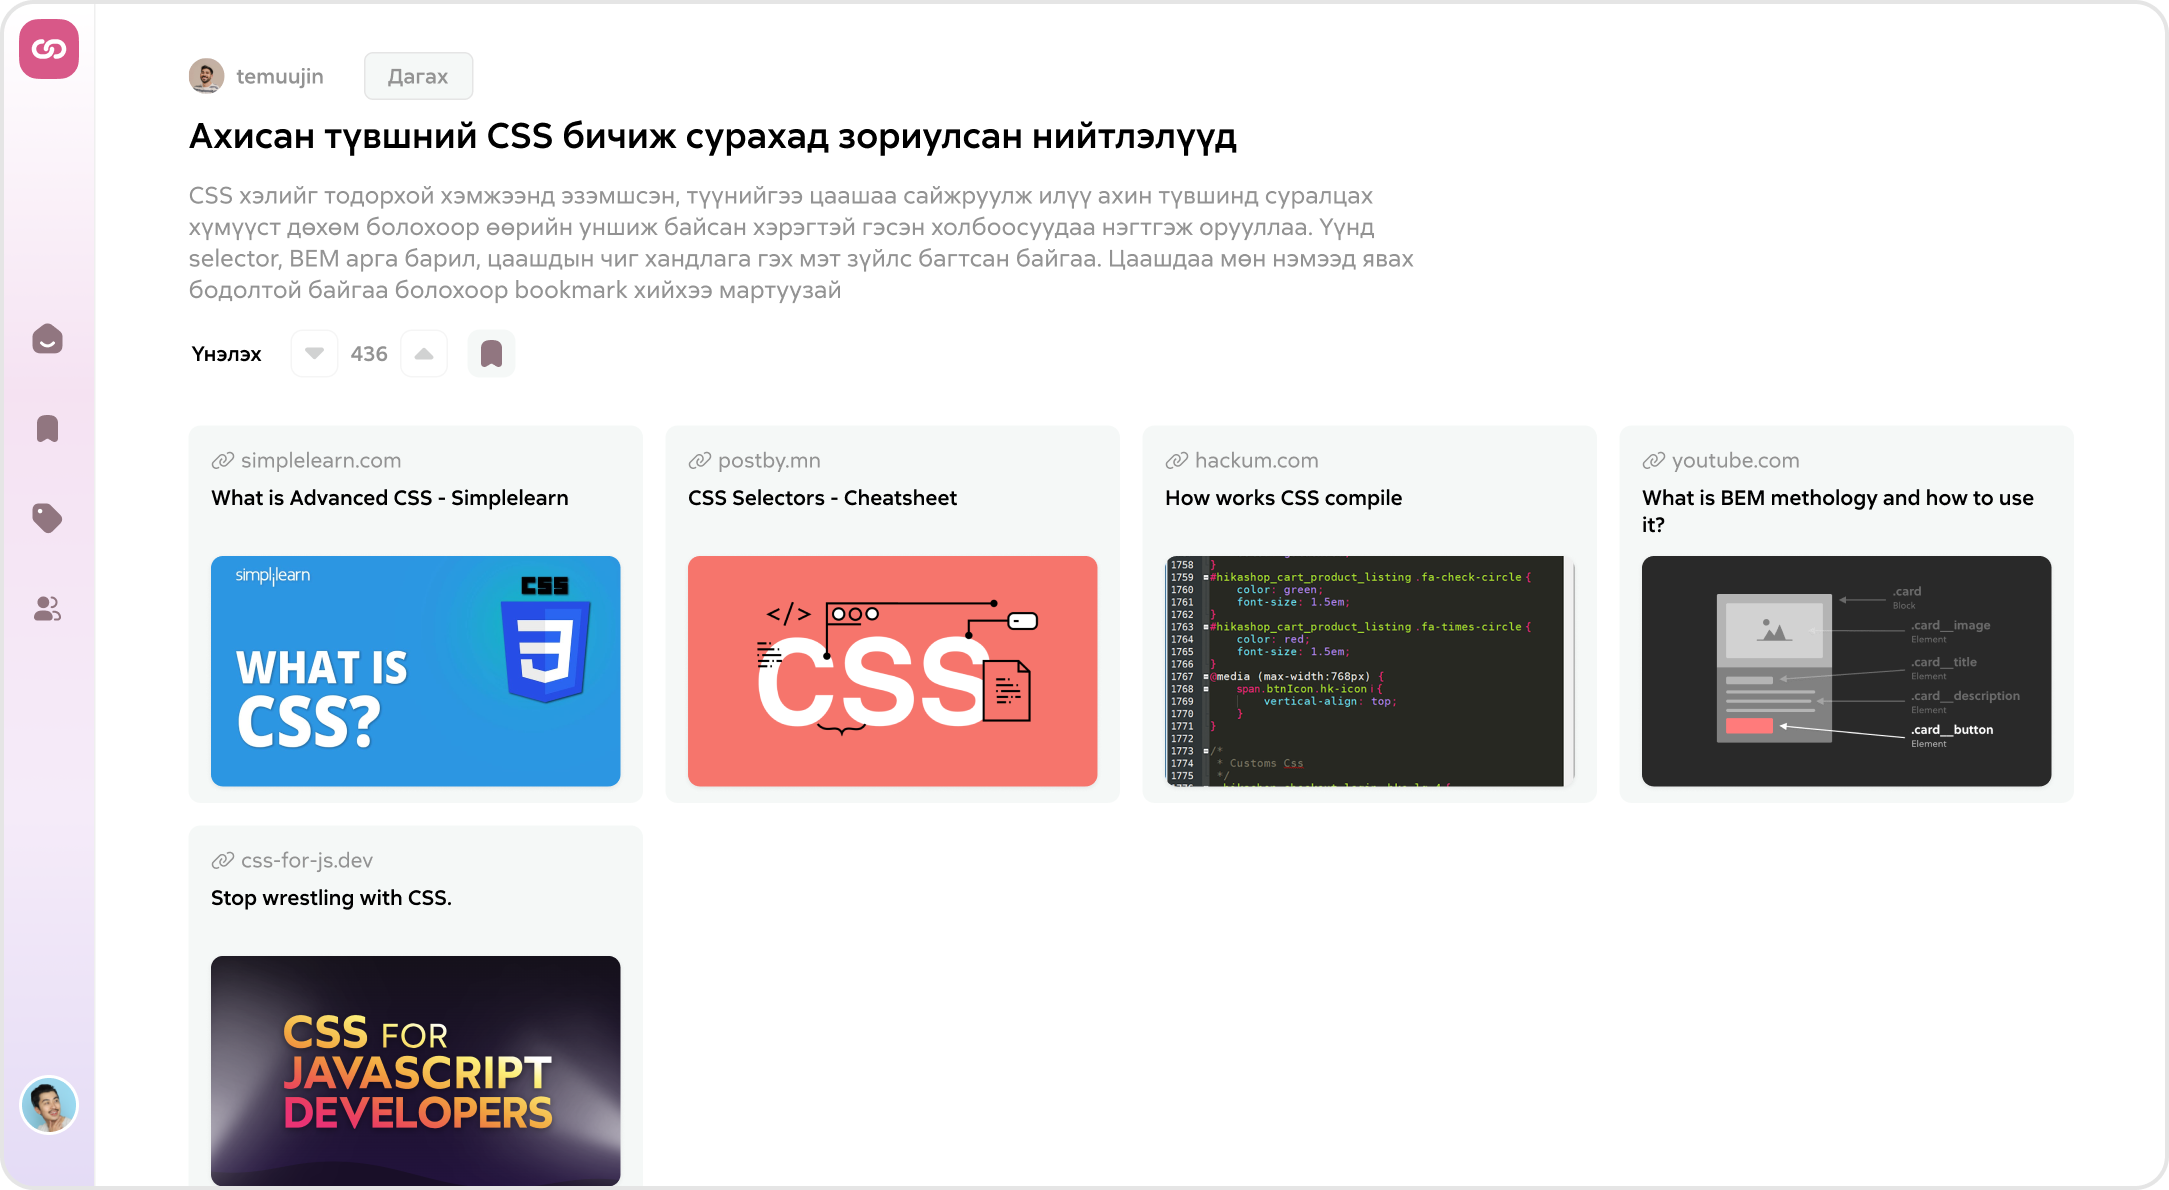
\includegraphics[width=10cm]{images/interfaces/grouped-link.png}
% 	\caption{Бүлэг холбоос доторх холбоосуудыг харах хуудас}
% 	\label{fig:grouped}
% \end{figure}

\clearpage
\section{Өгөгдлийн сан}

\subsection{Өгөгдлийн сангийн диаграм}
\begin{figure}[h]
	\centering
	\includesvg[width=15cm]{images/rd_schema.png}
	\caption{Системийн баазын бүтэц}
	\label{fig:erd}
\end{figure}

\pagebreak

\textbf{Уралдааны төрөл хадгалах өгөгдлийн баазын JSON}

\begin{figure}[h]
	\centering
	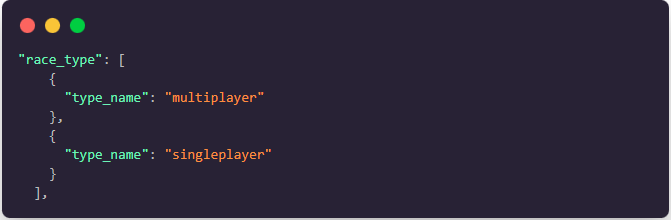
\includegraphics[width=15cm]{images/race_type_json.png}
	\caption{Хэрэглэгчийн үзүүлэлтийн жишээ дата}
	\label{fig:erd}
\end{figure}

\textbf{Уралдааны текст хадгалах өгөгдлийн баазын JSON}

\begin{figure}[h]
	\centering
	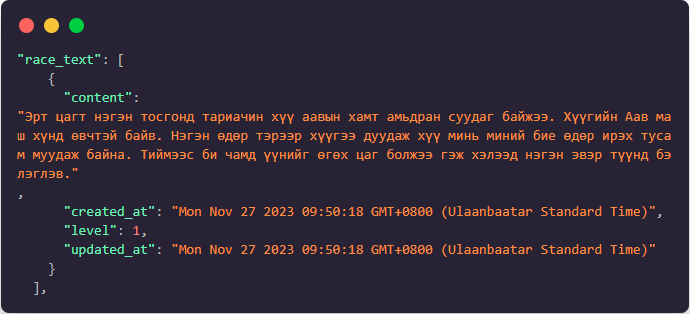
\includegraphics[width=15cm]{images/race_text_json.png}
	\caption{Хэрэглэгчийн үзүүлэлтийн жишээ дата}
	\label{fig:erd}
\end{figure}

\pagebreak

\textbf{Уралдаан хадгалах өгөгдлийн баазын JSON}

\begin{figure}[h]
	\centering
	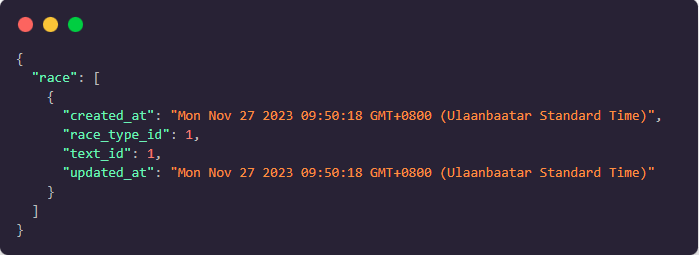
\includegraphics[width=15cm]{images/race_json.png}
	\caption{Уралдааны жишээ дата}
	\label{fig:erd}
\end{figure}

\textbf{Хэрэглэгчийн үзүүлэлтийг хадгалах өгөгдлийн баазын JSON}

\begin{figure}[h]
	\centering
	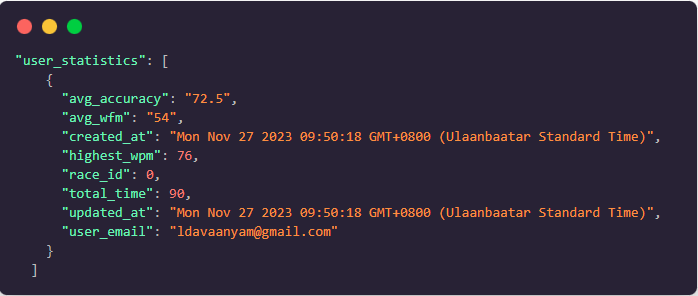
\includegraphics[width=15cm]{images/statistics_json.png}
	\caption{Хэрэглэгчийн үзүүлэлтийн жишээ дата}
	\label{fig:erd}
\end{figure}

\pagebreak
\textbf{Өгөгдлийн сангийн хүснэгтүүдийн тайлбар}

\begin{table}[h]
	\caption{User хүснэгт}
	\begin{tabular}{|l|l|l|p{8cm}|}
		\hline
		№ & Талбарын нэр & Өгөгдлийн төрөл & Тайлбар                                                                                    \\ \hline
		1 & id           & int             & Хэрэглэгчийн дахин давтагдашгүй ID-г хадгална - Auto Incremented                           \\ \hline
		2 & username     & varchar         & Хэрэглэгчийн гараас оруулж өгсөн нэрийг хадгална. Зөвхөн латин тэмдэгтүүд ашиглах хэрэгтэй \\ \hline
		3 & email        & varchar         & Хэрэглэгчийн цахим шуудан                                                                  \\ \hline
		4 & password     & varchar         & Хэрэглэгчийн гараас оруулж өгсөн нууц үгийг encrypt-лэж /hash/ уг хэсэгт хадгална          \\ \hline
		5 & profile\_img & link            & Хэрэглэгчийн оруулж өгсөн зургийг сервер дээр хадгалж, замыг нь энэ хэсэгт хадгална        \\ \hline
		6 & created\_at  & timestamp       & Хэрэглэгчийн хаяг үүссэн хугацааг серверээс авч хадгална                                   \\ \hline
		7 & updated\_at  & timestamp       & Хэрэглэгчийн хаяг өөрчлөгдсөн хугацаагсерверээс авч хадгална                               \\ \hline
	\end{tabular}
\end{table}

\begin{table}[h]
	\caption{User Statistics Table}
	\begin{tabular}{|l|l|l|p{8cm}|}
		\hline
		№  & Талбарын нэр   & Өгөгдлийн төрөл & Тайлбар                                                                       \\ \hline
		1  & id             & int             & Хэрэглэгчийн статистикийн дахин давтагдашгүй ID-г хадгална - Auto Incremented \\ \hline
		2  & user\_race\_id & int             & Хэрэглэгчийн статистикийг уралдааны хүснэгттэй Foreign Key-р хадгална         \\ \hline
		3  & user\_email    & int             & Хэрэглэгчийн статистикийг хэрэглэгчийн хүснэгттэй Foreign Key-р хадгална      \\ \hline
		4  & tests\_taken   & int             & Хэрэглэгчийн авсан тестийн нийт тоог хадгална                                 \\ \hline
		5  & avg\_wpm       & float           & Хэрэглэгчийн шивэх хурдны минутын дундаж үгийг хадгална.                      \\ \hline
		6  & avg\_accuracy  & float           & Хэрэглэгчийн шивэх дундаж нарийвчлалын хувийг хадгална                        \\ \hline
		7  & high\_wpm      & float           & Хэрэглэгчийн шивэх хурдад хүрсэн минутанд хамгийн их үгийг хадгална           \\ \hline
		8  & total\_time    & float           & Хэрэглэгчийн уралдаанд зохиулсан хугацааг хадгална                            \\ \hline
		9  & created\_at    & timestamp       & Хэрэглэгчийн хаяг үүссэн хугацааг серверээс авч хадгална                      \\ \hline
		10 & updated\_at    & timestamp       & Хэрэглэгчийн хаяг өөрчлөгдсөн хугацааг серверээс авч хадгална                 \\ \hline
	\end{tabular}
\end{table}

\begin{table}[h]
	\caption{Race Table}
	\begin{tabular}{|l|l|l|p{8cm}|}
		\hline
		№ & Талбарын нэр   & Өгөгдлийн төрөл & Тайлбар                                                                             \\ \hline
		1 & id             & int             & Уралдааны дахин давтагдашгүй ID-г хадгална - Auto Incremented                       \\ \hline
		2 & race\_type\_id & int             & Тэмцээний төрлийн хүснэгттэй Foreign Key-р хадгална                                 \\ \hline
		3 & text\_id       & int             & Тэмцээнд ашигласан текстийг зааж өгсөн race\_text хүснэгттэй Foreign Key-р хадгална \\ \hline
		4 & created\_at    & timestamp       & Хэрэглэгчийн хаяг үүссэн хугацааг серверээс авч хадгална                            \\ \hline
		5 & updated\_at    & timestamp       & Хэрэглэгчийн хаяг өөрчлөгдсөн хугацааг серверээс авч хадгална                       \\ \hline
	\end{tabular}
\end{table}


\begin{table}[h]
	\caption{Race Type Table}
	\begin{tabular}{|l|l|l|p{8cm}|}
		\hline
		№ & Талбарын нэр & Өгөгдлийн төрөл & Тайлбар                                                               \\ \hline
		1 & id           & int             & Уралдааны төрлийн дахин давтагдашгүй ID-г хадгална - Auto Incremented \\ \hline
		2 & type\_name   & varchar         & Тэмцээний төрлийн нэрийг хадгалах хувьсагчийн тэмдэгтийн багана       \\ \hline
	\end{tabular}
\end{table}

\begin{table}[h]
	\caption{Race Text Table}
	\begin{tabular}{|l|l|l|p{8cm}|}
		\hline
		№ & Талбарын нэр & Өгөгдлийн төрөл & Тайлбар                                                                               \\ \hline
		1 & id           & int             & Уралдааны өгүүлбэрийн дахин давтагдашгүй ID-г хадгална - Auto Incremented             \\ \hline
		2 & контент      & varchar         & Тэмцээний үеэр хэрэглэгчдийн шивэх бодит текстийг хадгалах хувьсах тэмдэгтийн багана. \\ \hline
		3 & level        & int             & Текстийн хүндрэлийн түвшинг харуулах бүхэл багана                                     \\ \hline
		4 & created\_at  & timestamp       & Хэрэглэгчийн хаяг үүссэн хугацааг серверээс авч хадгална                              \\ \hline
		5 & updated\_at  & timestamp       & Хэрэглэгчийн хаяг өөрчлөгдсөн хугацааг серверээс авч хадгална                         \\ \hline
	\end{tabular}
\end{table}



\clearpage





